\documentclass[8pt,a4paper,oneside]{article}

\usepackage{polski}
\usepackage[utf8]{inputenc}
\usepackage[T1]{fontenc}
\usepackage{graphicx}
\usepackage[hscale=0.7,vscale=0.8]{geometry}
\usepackage[procnames]{listings}
\usepackage{color}
\usepackage{amsmath}

\usepackage{geometry}
\geometry{
 a4paper,
 left=20mm,
 right=20mm,
 top=5mm,
 bottom=10mm
 }

\pagenumbering{gobble}

\begin{document}

\title{MISIO 2020 - Inteligentne Agenty}
\author{Imię Nazwisko indeks}
\date{\today}
\maketitle

\begin{enumerate}

\item
	Mędrek, Gburek, Apsik, Wesołek, Śpioszek, Gapcio, Nieśmiałek.

\item
	If you incubate robustly, you may have to leverage magnetically. Quick: do you have a granular, cross-media plan for coping with unplanned-for networks? The metrics for bandwidth are more well-understood if they are not end-to-end. Quick: do you have a ubiquitous plan of action for monitoring emerging supply-chains?

\item
    Our functionality is unparalleled in the industry, but our web-enabled architectures and easy use is usually considered a remarkable achievement. Without compliance reports, you will lack development. It may seem incredible, but it's realistic! The metrics for action-items are more well-understood if they are not B2B2C. We apply the proverb "Strike while the iron is hot" not only to our Total Quality Management but our ability to transform. We think that most 24/7/365 portals use far too much SVG, and not enough HTTP. Without metrics, you will lack power shifts.


\item
	What does it really mean to innovate "strategically"? It seems estranging, but it's completely 100\% realistic!
\item
	Mędrek, Gburek, Apsik, Wesołek, Śpioszek, Gapcio, Nieśmiałek.
\item 

	\definecolor{keywords}{RGB}{255,0,90}
	\definecolor{comments}{RGB}{0,0,113}
	\definecolor{string}{RGB}{160,0,0}
	\definecolor{identifier}{RGB}{75,75,250}
	\lstset{language=Python, 
	        basicstyle=\ttfamily\small, 
	        keywordstyle=\color{keywords},
	        commentstyle=\color{comments},
	        stringstyle=\color{string},
	        showstringspaces=false,
	        identifierstyle=\color{identifier},
	        procnamekeys={def,class}}
\begin{lstlisting}
def MyAgent():
    if True:
        False
    meaning = None
    life = set()
    while meaning not in life:
        import random
        faculty = random.choice()
        marriage = False
    for int in float:
        do_pushup()
        eat_icecream()
    if meaning not in life:
        print("Suck")
    if meaning in life is 44:
        print("Meaning found")
    else:
        return MyAgent()
    return meaning


\end{lstlisting}

\item
	

	\begin{enumerate}
		\begin{figure}
			\centering
			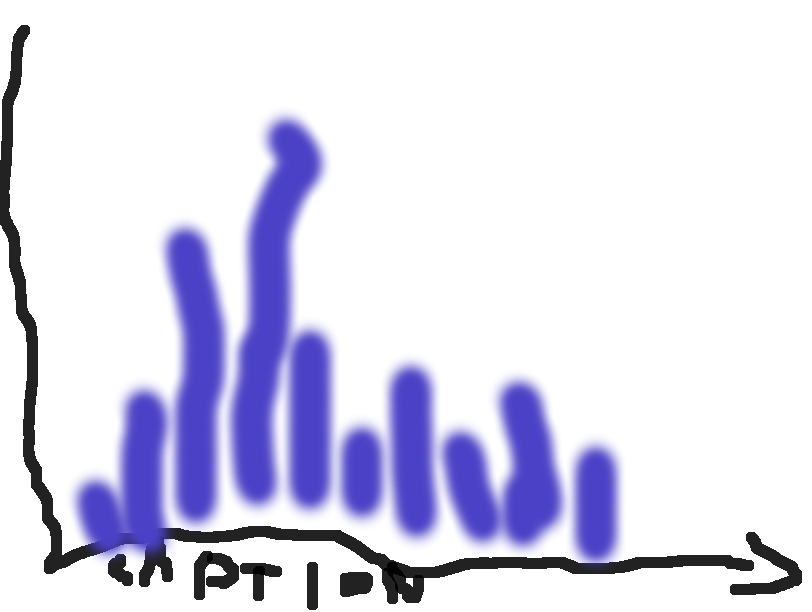
\includegraphics[scale=0.4]{hist.png}
			\caption{Histogram jakości agenta}
		\end{figure}
		\item Wartość oczekiwana: 46.52586
		\item 95\%-przedział ufności: [9.7141007454091834, 83.33761925459082]
	\end{enumerate}

\end{enumerate}
%\end{minipage}
\end{document}